% CVPR 2027 submission (built on the CVPR 2026 author kit); see https://github.com/cvpr-org/author-kit
\documentclass[10pt,twocolumn,letterpaper]{article}

\usepackage[review]{cvpr}      % REVIEW version (anonymous)

\usepackage{booktabs}
\usepackage{multirow}
\usepackage{amsmath,amssymb}
\usepackage{graphicx}
\usepackage{xcolor}
\usepackage{microtype}
%% This file contains a number of tweaks that are typically applied to the main document.
%% They are not enabled by default, but can be enabled by uncommenting the relevant lines.


%%
%% Official support for 2-column teaser figure
%%

%%
%% For auto-referencing of figures (see fig/teaser.tex and \label{} therein) 
%%
\usepackage{currfile} %< for \currfilebase macro

%%
%% caption and (global) spacing overrides
%%
\usepackage{caption} %< for "\captionof" commands (teaser)
% \setlength{\abovecaptionskip}{.5em} % space above caption
% \setlength{\belowcaptionskip}{1em} % space below caption

%%
%% Inline annotations; for predefined colors, refer to "dvipsnames" in the xcolor package:
%% https://tinyurl.com/overleaf-colors
%%
\newcommand{\red}[1]{{\color{red}#1}}
\newcommand{\todo}[1]{{\color{red}#1}}
\newcommand{\TODO}[1]{\textbf{\color{red}[TODO: #1]}}
%%
%% Disable for camera ready / submission by uncommenting these lines:
%%
% \renewcommand{\TODO}[1]{}
% \renewcommand{\todo}[1]{#1}

%%
%% Work harder in optimizing text layout. Typically shrinks text by 1/6 of page, enable
%% it at the very end of the writing process, when you are just above the page limit.
%%
% \usepackage{microtype}

%%
%% Fine-tune paragraph spacing.
%%
% \renewcommand{\paragraph}[1]{\vspace{.5em}\noindent\textbf{#1.}}

%%
%% Globally adjusts space between figure and caption.
%%
% \setlength{\abovecaptionskip}{.5em}

%%
%% Allows "the use of \paper to refer to the project name"
%% with automatic management of space at the end of the word.
%%
% \usepackage{xspace}
% \newcommand{\paper}{ProjectName\xspace}

%%
%% Commonly used math definitions.
%%
% \DeclareMathOperator*{\argmin}{arg\,min}
% \DeclareMathOperator*{\argmax}{arg\,max}

%%
%% Tighten underline.
%%
% \usepackage{soul}
% \setuldepth{foobar}

%%
%% Reconfigure paragraph (tweaks spacing)
%%


\definecolor{cvprblue}{rgb}{0.21,0.49,0.74}
\usepackage[pagebackref,breaklinks,colorlinks,allcolors=cvprblue]{hyperref}

\def\paperID{*****}
\def\confName{CVPR}
\def\confYear{2027}

\newcommand{\HI}{{\small\textsf{HI}}}
\newcommand{\MID}{{\small\textsf{MID}}}
\newcommand{\LO}{{\small\textsf{LO}}}
\newcommand{\pend}[1]{{\color{red}#1}}

\title{When Text Locks Out Vision: Measuring Visual Headroom in Multiple-Choice VQA}

\author{Anonymous CVPR submission\\
Paper ID \paperID}

\begin{document}
\maketitle
\begin{abstract}
Whether a model looks at the image is usually inferred from the average accuracy drop when the image is removed. That average hides when nonvisual evidence becomes so predictive that additional visual evidence stops helping. We study this competition in multiple-choice VQA, where a text-side shortcut can settle answers without the image. We define a benchmark's \emph{visual headroom} as the accuracy a model gains from the true image over its \emph{blind ceiling}, the best accuracy reached without the image or from option text alone. We measure headroom with counterfactual images, a ladder of image strength, and a length shortcut planted at graded strength, so that shortcut strength and image strength vary jointly. Planting the shortcut lowers the image benefit on PMC-VQA from $+13.5$ to $+0.1$ points. The strength at which the image stops mattering depends on the benchmark: $0.85$ for Qwen-3B on PMC-VQA and $0.99$ on A-OKVQA. A boundary prediction fixed before its runs held for two further models, and three attempts to explain the difference between benchmarks failed. Without planting, headroom is $-0.1$ points on Med-CMR and $+4.9$ on OmniMedVQA, against $+13.7$ and $+33.2$ on PMC-VQA and A-OKVQA. On Med-CMR the shortest option is correct for $91.9\%$ of questions. For Qwen2.5-VL-3B, fine-tuning on the benchmark's own training split installed this shortcut within about 1{,}000 questions (two seeds, one benchmark) and left no measurable headroom. A penalty on confident answers under a mismatched image restores measurable image dependence for $4$ to $6$ points of accuracy. The restored dependence is partly coarse: the same penalty loses $11$ to $18$ points against a plausible wrong image. We report failed and post-hoc tests, and all tests follow dated, hash-chained amendments.
\end{abstract}

\section{Introduction}
\label{sec:intro}

\begin{figure*}[t]
  \centering
  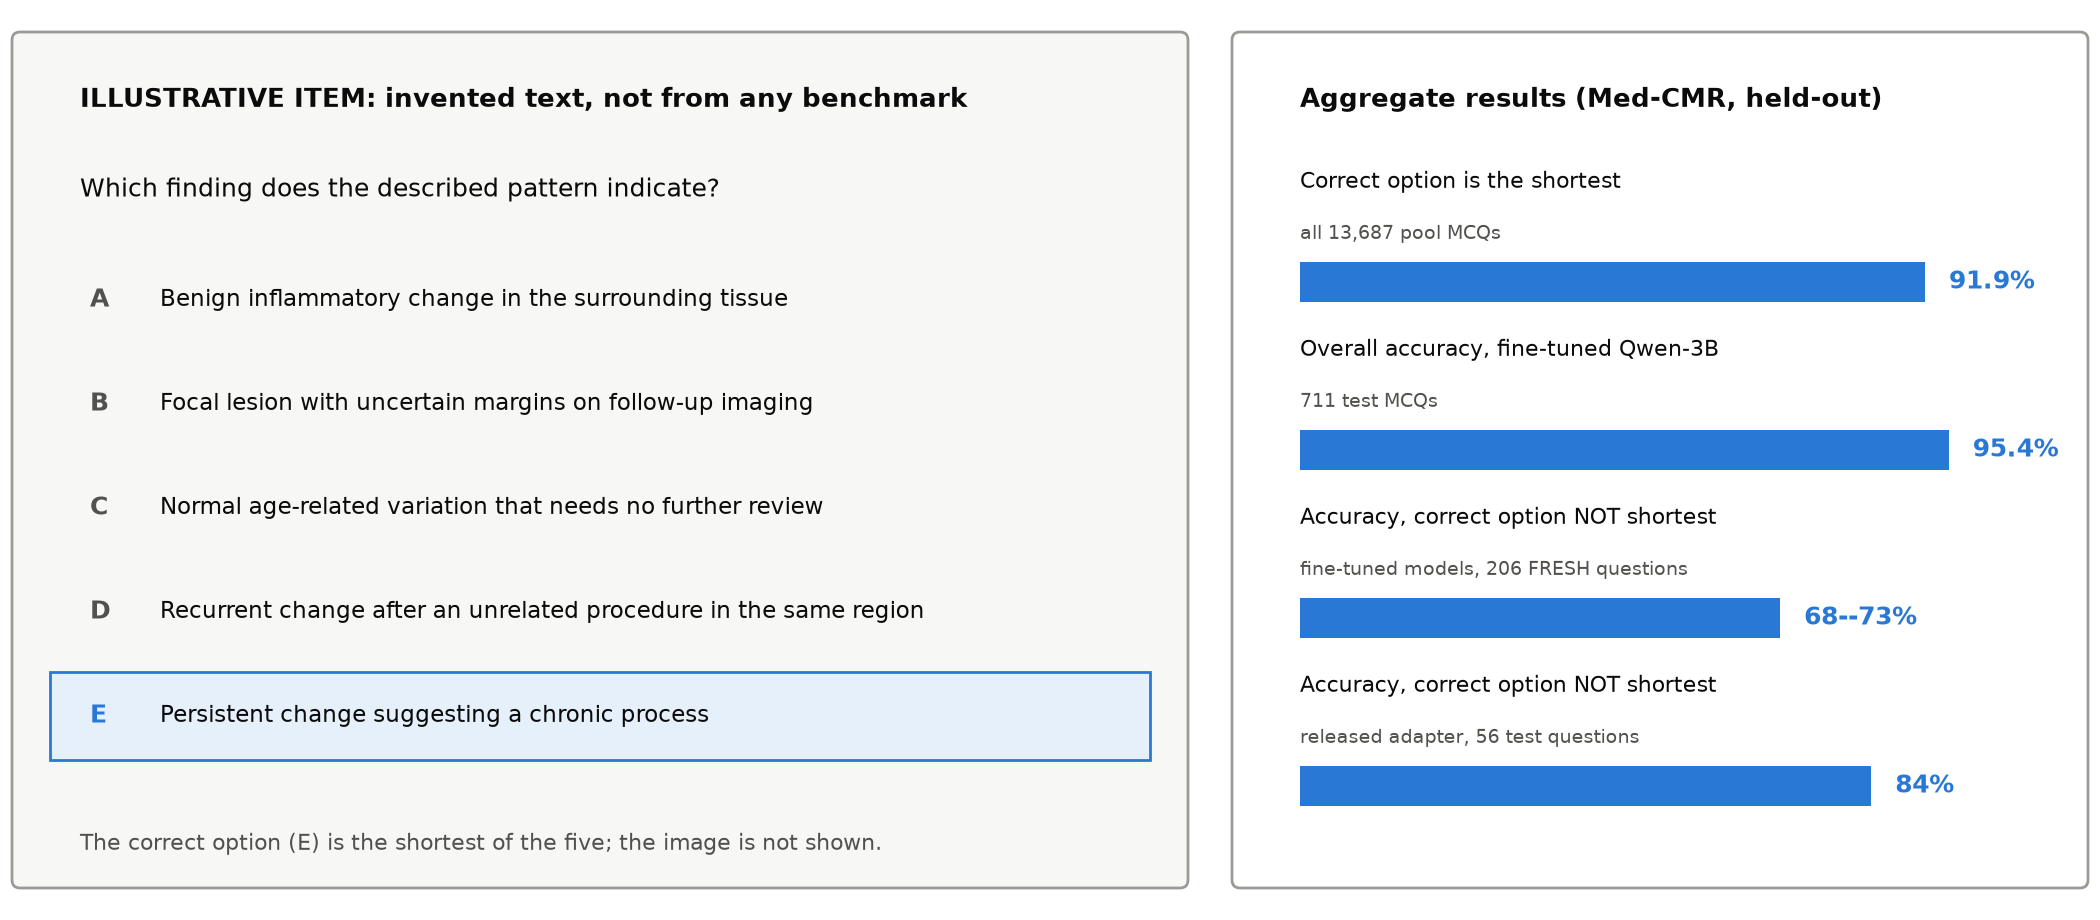
\includegraphics[width=0.76\textwidth]{fig/f1_teaser_illustrative.png}
  \caption{\textbf{An illustrative item and the aggregate numbers it summarises.} The item and its options are invented for illustration and are not from any benchmark; no image is shown. The bars report measured aggregates on Med-CMR: the correct option is the shortest in 91.9\% of the 13{,}687 pool questions; overall accuracy is 95.4\% for fine-tuned Qwen-3B (711 test questions) and 96.1\% for the released adapter; where the correct option is not the shortest, accuracy is 68.0\% and 73.3\% for fine-tuned Qwen-3B and Qwen-7B (206 FRESH questions) and 83.9\% for the released adapter (56 test questions). The bar lengths are schematic.}
  \label{fig:teaser}
\end{figure*}

Studies of medical imaging models have repeatedly reported accuracy that did not rest on disease: COVID-19 chest X-ray models relied on confounding factors and failed in new hospitals~\cite{degrave2021shortcuts}; a pneumonia model performed worse at outside hospitals and could identify a radiograph's source hospital in over 99.9\% of cases~\cite{zech2018variable}; the specificity of a deep learning melanoma classifier fell from 84.1\% to 45.8\% on lesions with surgical skin markings~\cite{winkler2019markings}; and a deployed retinopathy screener met image-quality demands that clinics could not always satisfy~\cite{beede2020humancentered}.
A 2026 preprint reports that frontier models describe images that were never provided and that a text-only model ranked first on a chest X-ray question-answering benchmark~\cite{asadi2026mirage}.
Training on benchmark data can raise scores without the ability~\cite{zhou2023cheater,zhang2024gsm1k}; Figure~\ref{fig:teaser} illustrates the pattern with an invented item; the numbers it summarises are measured on the benchmark, where the training split is the source of the shortcut.
Do vision-language models look at the image?
Audits of medical VQA say mostly not: tuned models lose few points when the image is blanked or swapped~\cite{zafar2026coral}, models ``derive more useful information from the question text than from the image''~\cite{pokrywka2026polish}, and the answer options alone carry exploitable cues~\cite{wang2026medqamm}.
These findings are usually summarised by one number, the average accuracy drop without the image, and read as ``the model ignores the image''.
That number answers the wrong question.
The question that matters is when nonvisual evidence becomes so predictive that additional visual evidence stops helping, and what that leaves for vision to earn.
We call the credit that vision can still earn the benchmark's \emph{visual headroom}: the accuracy of a model with the true image above what it reaches without the image or from option text alone (the \emph{blind ceiling}).
We separate four things that are easily conflated: whether visual information is available (the image is given); whether predictions depend on it (counterfactual images change the answer); whether predictions are accurate because of it (the image adds accuracy above the blind ceiling, which is headroom); and whether the model reasons about the relevant visual content (the right image and region). We test the second throughout and the third through headroom; the fourth is tested only in part (wrong-image identity, blur, occlusion), and we make no claim of semantic understanding.

We answer in six steps, one per section, each about headroom: \textbf{Failure} (Sec.~\ref{sec:obs}): accurate Med-CMR systems have none, on a benchmark whose correct option is the shortest in 91.9\% of the questions; \textbf{Isolation} (Sec.~\ref{sec:setting}): the blind ceiling, counterfactual images, a ladder of image strength and planted shortcuts; \textbf{Quantification} (Sec.~\ref{sec:dose}): planting a shortcut dials headroom from $+13.5$ to $+0.1$ points, at a strength that depends on the benchmark; \textbf{Explanation} (Sec.~\ref{sec:explain}): the cue is sufficient but not the only consumer (option wording and prior knowledge are others); \textbf{Intervention} (Sec.~\ref{sec:remedy}): headroom can be partly bought back for about 4 to 6 points of accuracy, and the bought-back dependence is partly coarse; \textbf{Stress test} (Sec.~\ref{sec:general}): a held-out prediction, the failures and an audit of the challenge's faithfulness judge.
Sec.~\ref{sec:setting} is the method and Secs.~\ref{sec:dose}--\ref{sec:general} are the experiments.

\paragraph{Contributions.}
(i)~A controlled two-axis characterization of the competition between shortcut and visual evidence: image benefit against shortcut strength and image strength (a phase diagram) in a medical and a natural-image benchmark, with a benchmark-dependent lock-out strength ($0.85$ against $0.99$ for Qwen-3B; the first from a grid fixed in advance, the second from a grid extended after a failed prediction, Sec.~\ref{sec:dose}) reported as a measured finding, not a law.
(ii)~What held and what did not: a prediction fixed before the runs held for two further models; three attempts to explain the boundary across benchmarks failed (the benefit without a cue, a one-constant evidence-competition hypothesis, natural variation in text predictability).
(iii)~The visual headroom of four benchmarks (blind ceiling, counterfactual images, a strength ladder): Med-CMR ($-0.1$ points) and OmniMedVQA ($+4.9$) leave almost none, PMC-VQA $+13.7$ and A-OKVQA $+33.2$; average measures rank systems inconsistently.
(iv)~What consumes headroom on Med-CMR and what buying it back costs: the length cue (installed by training on about 1{,}000 questions of the benchmark's own split), wording that resembles the distractors, 96\% overall but 68--73\% (our models) and 84\% (the released system) where length misleads (ids released); about 4 to 6 points of accuracy at 3B and 7B, after ten earlier attempts that did not meet their criteria (Supp.~X), and 11 to 18 points against a plausible wrong image; faithfulness judges that penalise a missing image only when the trace says so.
All tests follow dated, hash-chained amendments (A0--A44), post-hoc criteria are marked and failures are reported.

\section{Related Work}
\label{sec:related}

\paragraph{Shortcuts and language priors.}
Image-blind answers have been studied since VQA~v2 was built to balance them~\cite{goyal2017making}; prior-robust training~\cite{agrawal2018dont}, shortcut benchmarks~\cite{si2022language} and the general account of shortcut learning~\cite{geirhos2020shortcut} followed; for multiple choice, hypothesis-only and option-only baselines~\cite{poliak2018hypothesis,gururangan2018annotation} and easy-option bias~\cite{zhang2025easyoption} show that options leak the answer.
Debiasing trains against a known bias, by ensembling with a biased expert~\cite{clark2019dont} or re-weighting examples~\cite{cadene2019rubi}; we use the former as a remedy whose effect we can attribute in a dose-controlled setting.

\paragraph{Shortcuts in medical VQA.}
Classic and large medical VQA sets~\cite{lau2018vqarad,liu2021slake,he2020pathvqa,zhang2023pmcvqa,hu2024omnimedvqa} are widely used, and recent audits question what they measure: MedQA-MM finds length-gap and wording cues in six medical MCQ datasets~\cite{wang2026medqamm}, a Polish board-exam benchmark finds models draw more from the text than the image~\cite{pokrywka2026polish}, SurgCheck shows task-dependent reliance on linguistic shortcuts~\cite{shin2026surgcheck}, and a counterfactual grounding study reports that image substitution costs at most 6.5 points on medical benchmarks~\cite{zafar2026coral}.
These works ask \emph{whether} models use the image on average; we ask under which shortcut and image strength, and we intervene.

\paragraph{Training on benchmarks.}
Training on benchmark-related data can raise scores without the ability: leaked evaluation data dramatically boosts results~\cite{zhou2023cheater}, some model families score up to 8\% lower on a fresh matched arithmetic set~\cite{zhang2024gsm1k}, multimodal models answer image-dependent questions without the image, which suggests memorized samples~\cite{chen2024mmstar}, and a 2026 preprint audit of medical VLM benchmarks finds overlap signals that manual review did not confirm as duplicates~\cite{xu2026medvlmaudit}.
We study the counterpart that needs no leakage: what a benchmark's own training split teaches.

\paragraph{Concurrent work and sample-level dependence.}
MIRAGE~\cite{asadi2026mirage} shows that frontier models describe and answer for images never provided and that a text-only model tops a chest X-ray VQA benchmark, .
Visual Information Gain~\cite{lee2026vig} scores how much visual input reduces prediction uncertainty for each training sample, a second preprint analyses how predictions respond to losing fine-grained visual evidence~\cite{lan2026seeing}, counterfactual probing with blank and mismatched images~\cite{zhu2026ask4vg} and designs crossing image presence with text integrity~\cite{senoglu2026sure} also measure image dependence, and audits of vision-indispensable subsets use multimodal gain and leakage~\cite{chen2024mmstar}.
We add a text-only blind ceiling and headroom per benchmark, shortcuts planted at graded strength (the cause and its dose), the released challenge system's accuracy where cleaning matters, an audit of its faithfulness judge, and an intervention with its price.

\section{Failure (Motivation): Accurate Systems With No Visual Headroom}
\label{sec:obs}

On Med-CMR~\cite{gong2025medcmr}, the benchmark of the MedReason~2026 challenge~\cite{medreason2026}, the correct option is the shortest of the five in 91.9\% of 13{,}687 questions (95\% CI 91.4--92.4), so a rule that picks it scores 91.1\% on the test slice.
Three benchmark-tuned model families (the released adapter of a top-3 system; Qwen2.5-VL and InternVL3 models that we fine-tune on the training split and evaluate on 3{,}000 questions they never saw) are \emph{text-saturated}: they stay confident when the image is replaced by a black one for 82--84\% of the questions, and on these \emph{text-decisive} questions no counterfactual image, whether black, random or a plausible wrong one, changes any answer (0 of 2{,}518, 2{,}503 and 2{,}463 questions, one count per system).
Fine-tuning installs the habit (the shortest option is picked 23--25\% of the time before and 91--92\% after), and the headline true-vs-black gaps of the three systems are within 1.3 points, so a conventional ablation calls them equally image-blind.
The stratified view tells them apart: on the 5--15\% text-undecided questions the released adapter gains $+12.1$ points from the image ($p=2\times10^{-5}$; on data that may overlap its unknown training set), whereas our fine-tuned models gain between $-4.1$ and $+2.6$ points across seven training configurations (Supp.~G).
High accuracy is therefore no evidence that these systems use the image, and the average drop without it hides where the image can matter at all.
The finding does not depend on this model-based stratifier: in terciles of a text-only option classifier that uses neither the model nor any image, at most 0.2\% of the answers in the most text-predictable third change under any counterfactual image (Supp.~Z).
Overall accuracy also hides where the cue points away; the released system keeps $83.9\%$ ($[73.2,92.9]$) on the 56 held-out questions whose correct option is not the shortest against $97.1\%$ on the others, our fine-tuned models lose more: on the 206 FRESH questions whose correct option is not the shortest, accuracy is $68.0\%$ (interval $[61.6,74.3]$; Qwen-3B) and $73.3\%$ ($[66.5,79.1]$; Qwen-7B) against $97.5$--$97.7\%$ on the others, and a black image changes it by about a point (Supp.~Z).
A text-only audit of seven multiple-choice sets (Supp.~Z) finds the length cue only in Med-CMR (the shortest-option rule scores 91.9\% against 20\% chance; the other sets are within 6 points of chance), but an option-only classifier that sees neither the question nor the image, the \emph{blind ceiling}, reaches 93.7\% on Med-CMR and 94.1\% on OmniMedVQA against 23--40\% on PMC-VQA, A-OKVQA, MedXpertQA-MM and MMMU health: saturation by text alone is not unique to Med-CMR, but it is far from general; the next section isolates what drives it.

\section{Isolation (Method): Protocol and Planted Shortcuts}
\label{sec:setting}

\paragraph{Readout and counterfactual images (protocol figure: Supp.~Z).}
We read the log-probabilities of the option letters at the answer position, take the arg\,max as the prediction and the margin (top-1 minus top-2 probability) as the confidence.
Each question is run with the true image and with counterfactuals: a black image, the image of another question, and the nearest-neighbour image (PubMedCLIP~\cite{eslami2023pubmedclip}), a plausible wrong one.
\emph{Text saturation} is the margin $m_b$ with the black image; with $\tau$ the 15th percentile of the margins of 700 unlabeled validation questions, a question is \HI{} (text-decisive) if $m_b\ge\tau$, \LO{} (text-undecided) if $m_b<0.90$ and \MID{} otherwise.
The \emph{image benefit} is $g=\mathrm{acc}(\text{image})-\mathrm{acc}(\text{black image})$ (points); an \emph{override} is a prediction that differs from the black-image answer.
The \emph{blind ceiling} of a benchmark is the accuracy of an option-level classifier that sees neither the question nor the image, and its \emph{visual headroom} is the true-image accuracy of a fine-tuned model minus the larger of its black-image accuracy and the blind ceiling (Supp.~Z).

\paragraph{Visual ladder and planted shortcuts.}
To vary the visual evidence we replace the true image by Gaussian blurs of radius 32, 16, 8, 4 and 2\,px (on the 448\,px image) and by the intact image.
To vary the shortcut we plant a neutral nonvisual cue at a controlled strength $d$, the share of questions in which the correct option carries it: neutral filler words on all options so that the correct option is the shortest (\emph{length}), or the correct option placed at position A (\emph{position}); training and test options are planted alike, the realised rate equals $d$ to within one question, and $d=0.25$ is a control that carries the same filler without a cue.

\paragraph{Benchmarks and systems.}
\emph{Med-CMR}: 14{,}398 five-option training MCQs, a frozen 711-question test slice and a pool of 16{,}836 further cases for fresh samples (case-disjoint and near-duplicate-filtered; no patient identifiers exist).
\emph{PMC-VQA}~\cite{zhang2023pmcvqa}: four-option questions on PubMed Central figures (9{,}277 training, 1{,}999 clean test, 3{,}000 held-out).
\emph{OmniMedVQA}~\cite{hu2024omnimedvqa} (open-access subset) and \emph{A-OKVQA}~\cite{schwenk2022aokvqa} (photographs; the 1{,}145 validation questions are the test set).
Systems: the released adapter of a top-3 MedReason~2026 system (Qwen3.5-9B, 4-bit, rank-16 LoRA~\cite{hu2022lora}; test accuracy 683/711 reproduced) and public models fine-tuned by us with one recipe: Qwen2.5-VL-3B and -7B~\cite{bai2025qwen25vl} and InternVL3-2B~\cite{zhu2025internvl3} (LoRA $r{=}16$ on the language layers, one epoch, learning rate $10^{-4}$, images at most 448\,px, loss on the answer letter).
All experiments follow one pre-specification with dated amendments, each frozen and SHA-256-hashed before the run it governs (the hashes are self-held, not an external registry); criteria fixed after earlier results are marked where they occur, and failed and not-evaluable tests are reported.

\begin{figure*}[t]
  \centering
  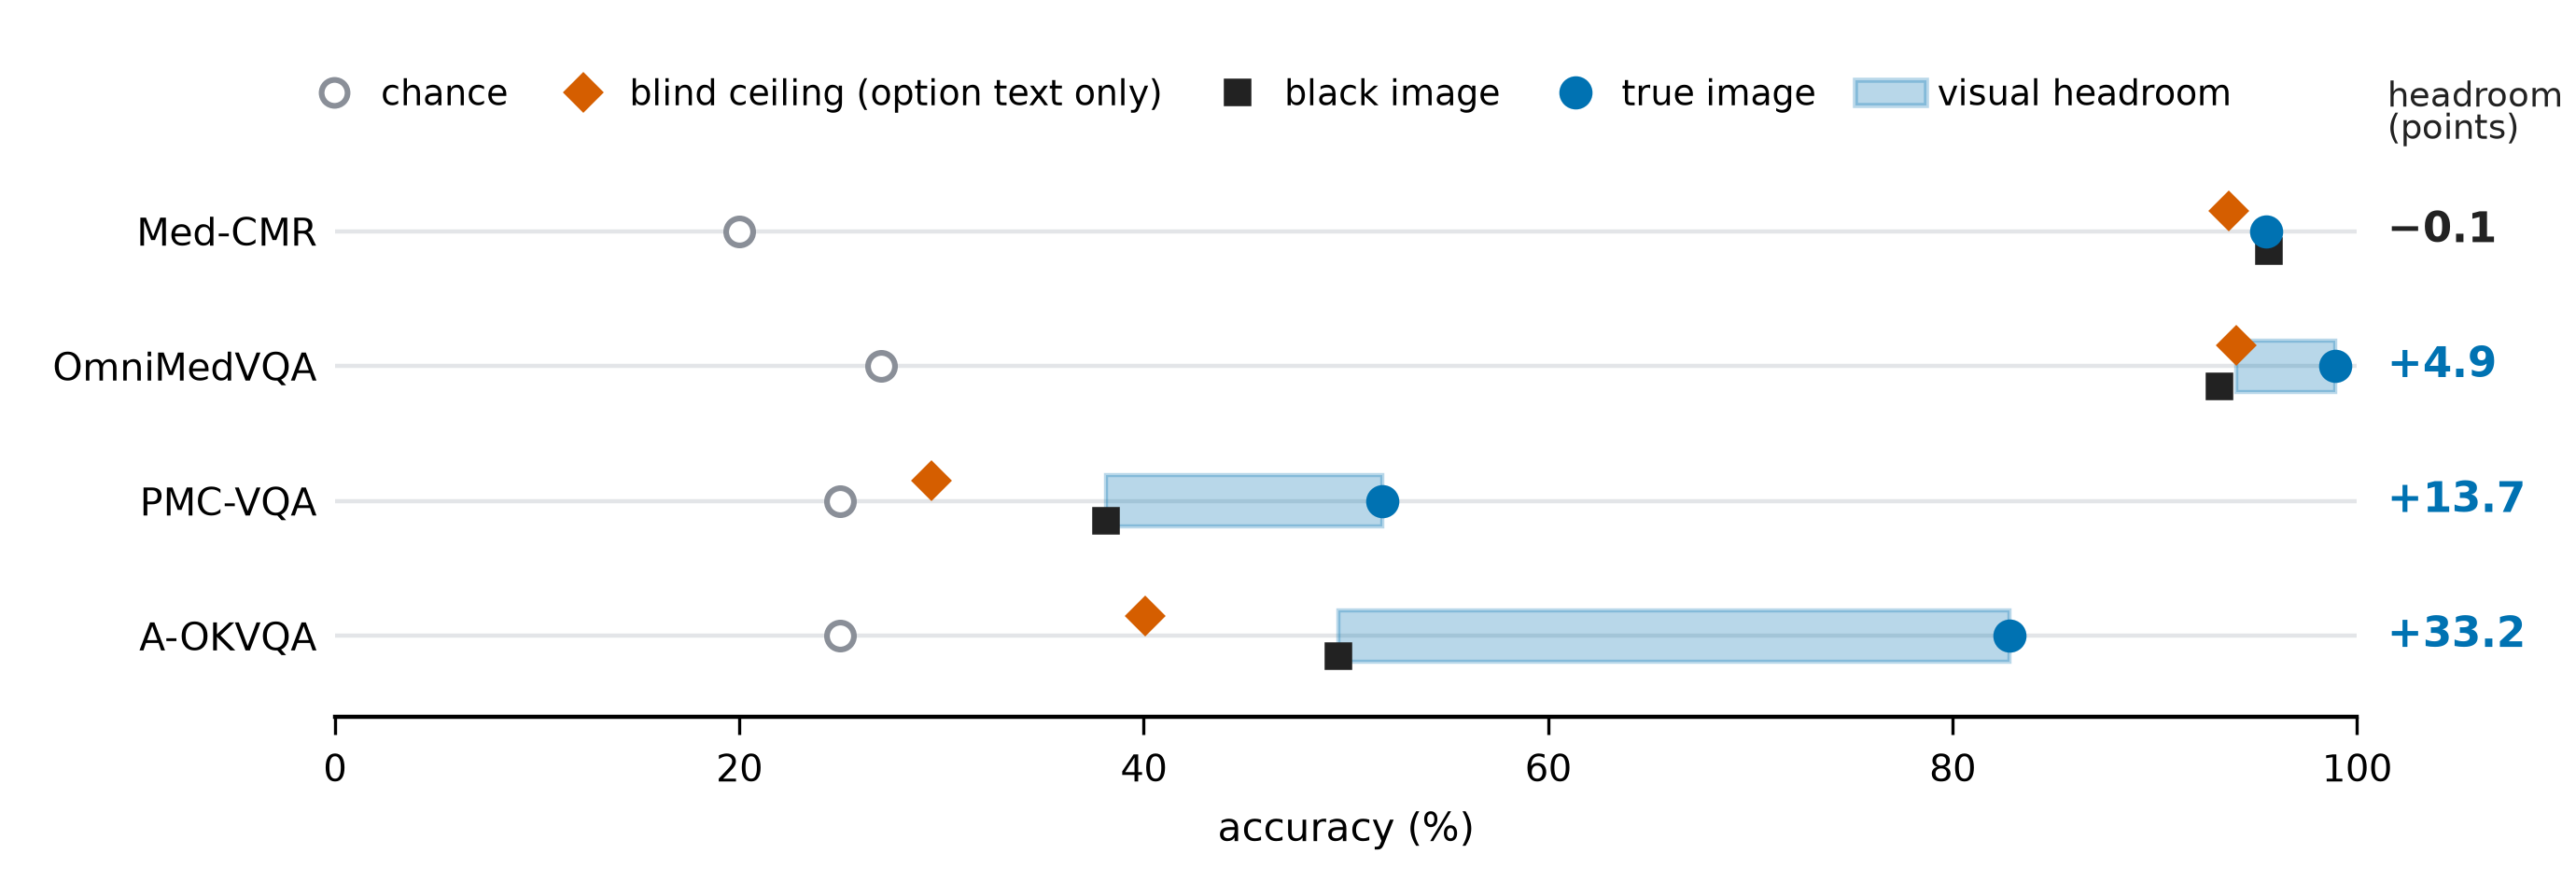
\includegraphics[width=0.74\textwidth]{fig/f2_headroom.png}
  \caption{\textbf{Visual headroom of four benchmarks} (fine-tuned Qwen2.5-VL-3B, held-out questions). Chance, the blind ceiling (an option-level classifier that sees neither the question nor the image), and the accuracy with a black image and with the true image; the shaded interval is the true-image accuracy above both no-image marks, i.e.\ the visual headroom (points, right).}
  \label{fig:headroom}
\end{figure*}

\paragraph{A contrast, observational.}
Headroom differs widely (Fig.~\ref{fig:headroom}): $-0.1$ points on Med-CMR (blind ceiling $93.7\%$), $+4.9$ on OmniMedVQA ($94.1\%$, with no length cue; we did not test why its blind ceiling is high), $+13.7$ on PMC-VQA ($29.5\%$) and $+33.2$ on A-OKVQA ($40.1\%$; fine-tuned Qwen-3B, Supp.~Z).
On PMC-VQA the correct option is the shortest in only 19.7\% of the questions; the same three families with the identical recipe do not acquire the habit (24--27\%), are never text-decisive (no black-image margin of at least $0.99$, against 75--79\% on Med-CMR) and lose $13.7$, $14.9$ and $14.4$ points without the image (Supp.~Z).
The benchmarks differ in topic and style, so this contrast is observational; planting the shortcut is the controlled test (Sec.~\ref{sec:dose}).

\section{Quantification (Experiments): Planting a Shortcut Dials Headroom Down}
\label{sec:dose}

\paragraph{Design.}
In PMC-VQA, where the correct option is not the shortest, we plant the length shortcut at $d\in\{0.25,0.40,0.55,0.70,0.85,0.92\}$ and fine-tune Qwen2.5-VL-3B for each dose and three seeds (18 runs); we evaluate on the 1{,}999 clean test questions with the true image, a black image and the six-level visual ladder.
We define the \emph{visual veto boundary} $V^\ast$ as the weakest ladder level at which the image benefit $g$ reaches $+2$ points with a paired-bootstrap lower bound of at least $+1$; $V^\ast=\text{none}$ if no level qualifies (criterion fixed before the runs).

\paragraph{Three quantities, not to be confused.} The visual veto boundary $V^\ast$ and the \emph{lock-out} (the weakest tested shortcut strength at which $V^\ast$ is \emph{none}) were fixed before the PMC-VQA dose study (amendment A17), and the PMC-VQA lock-out of $0.85$ comes from that pre-specified grid. The A-OKVQA lock-out at $0.99$ is different: the criterion was fixed before the runs, but the strength was added after the $0.92$ prediction failed (A21, A22; Supp.~W). The $20\%$ relative criterion, the strength at which the benefit falls to a fifth of its value at $d=0.25$, is exploratory (Supp.~Y): it gives lower strengths ($0.74$ for Qwen-3B on PMC-VQA; $0.94$ on A-OKVQA) and is not a lock-out.

\begin{figure*}[t]
  \centering
  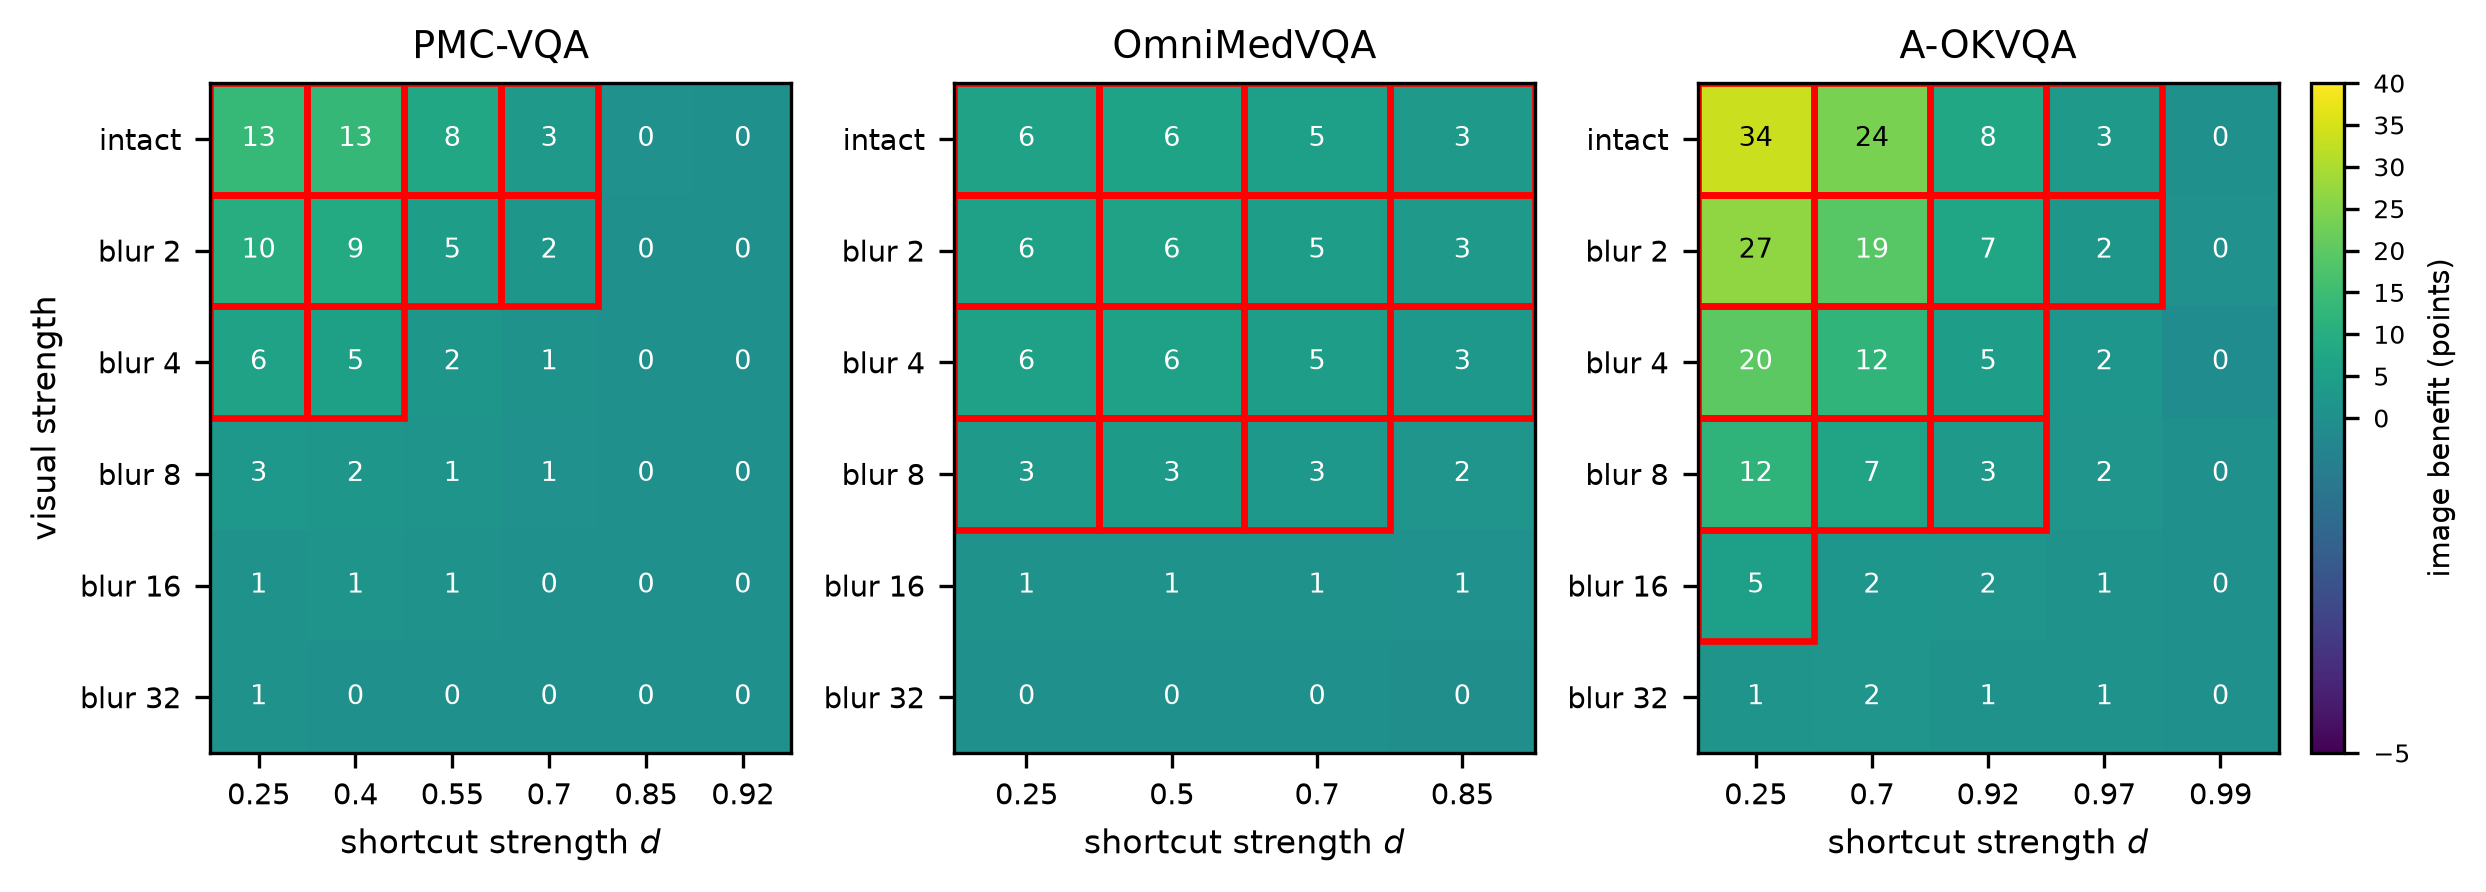
\includegraphics[width=0.78\textwidth]{fig/f12_phase.png}
  \caption{\textbf{Phase diagram of image use} (planted length shortcut, Qwen2.5-VL-3B; mean of 2--3 seeds; test sets of 1{,}999, 2{,}000 and 1{,}145 questions). Cells: image benefit, the accuracy with the image at the visual strength of the row (Gaussian blur radius 32, 16, 8, 4, 2\,px on 448\,px images, or intact) minus the accuracy with a black image, in points; columns: the tested shortcut strengths $d$ of each benchmark. Red outline: the visual-veto criterion holds in every seed, i.e.\ the benefit is at least $+2$ points with a paired-bootstrap 95\% lower bound of at least $+1$. A column without outline is a lock-out; it is bracketed by the tested strengths, not fitted: PMC-VQA is locked from $d=0.85$ (unlocked at $0.70$), A-OKVQA at $0.99$ (unlocked at $0.97$), OmniMedVQA is not locked up to $0.85$ (the highest tested).}
  \label{fig:phase}
\end{figure*}

\begin{figure*}[t]
  \centering
  \includegraphics[width=\textwidth]{fig/f10_domains.pdf}
  \caption{\textbf{Shortcut strength and visual control in two domains} (planted length shortcut). (a)~Image benefit of the intact image against the shortcut strength $d$ (logit scale), PMC-VQA (blue; Qwen-3B three seeds, InternVL3-2B and Qwen-7B two seeds) and A-OKVQA (green; Qwen-3B three seeds, Qwen-7B and InternVL3-2B two seeds). (b)~Veto boundary $V^\ast$ (mean over seeds; \emph{none}: no tested image strength helps). (c,d)~Benefit along the visual ladder (Qwen-3B): where the shortcut is strong the image helps only when it is intact or nearly so, or not at all.}
  \label{fig:dose}
\end{figure*}

\paragraph{The image benefit falls with the dose.}
On PMC-VQA the benefit of the intact image falls monotonically from $+13.5$ points at $d=0.25$ to $+13.2$, $+8.0$, $+3.4$, $+0.4$ and $+0.1$ points at $d=0.92$ (Fig.~\ref{fig:dose}a; pooled Spearman $\rho=-0.96$, permutation $p<10^{-4}$, Holm-corrected; every seed $\rho\le-0.94$).
At the same time the model learns the shortcut (picks the shortest option 22\%, 42\%, 75\%, 92\%, 99\%, 99\% of the time), its text-side margin rises from $0.25$ to $3.25$ log-odds, and its accuracy on the original, cue-free options falls from 52\% to 38\% (Supp.~Q).
The veto boundary shifts with it (Fig.~\ref{fig:dose}b,c): at $d=0.25$ a blur of radius 8 or 4 already gives a benefit; at $d=0.55$--$0.70$ only a blur of radius 4 or 2 does; for $d\ge0.85$ no image strength qualifies (none in all three seeds; $\rho(d,V^\ast)=+0.94$, Holm-corrected).

\paragraph{The same intervention on natural photographs.}
On A-OKVQA the correct option is the shortest in only 16.1\% of the test questions.
Between $d=0.25$ and $0.92$ the benefit falls from about $+34$ to $+8$ points (Qwen-3B $+33.9\to+8.1$, Qwen-7B $+34.2\to+6.5$, InternVL3-2B $+37.6\to+11.7$).
At $d=0.97$ and $0.99$, tested after seeing this with criteria fixed beforehand, the benefit of Qwen-3B is $+2.5$ to $+3.3$ and $+0.1$ to $+0.35$ points with no helpful image strength in three seeds, and Qwen-7B behaves alike; InternVL3-2B keeps $+1.7$ points at $0.99$.
The lock-out strength is thus not a constant ($0.85$ for Qwen-3B on PMC-VQA, $0.99$ for the Qwen models on A-OKVQA) and is not ordered by the benefit without a cue (Sec.~\ref{sec:general}; Supp.~Y).
A position shortcut and a centre-versus-border occlusion are in Supp.~Q and Z; attempts to explain the boundary are in Sec.~\ref{sec:general}.

\section{Explanation (Analysis): What the Cue Explains, and What It Does Not}
\label{sec:explain}

\paragraph{A strong cue is sufficient.}
Where the shortcut is weak the image can still change the decision and its benefit grows with its strength; where the shortcut is reliable enough, visual evidence of any tested strength stops affecting accuracy and the decision is \emph{locked} by the text side.
That a model fine-tuned on a reliable cue comes to rely on it is the expected direction; what the study measures is how the decision and the weakest helpful image change with the cue strength, and that the lock-out strength moves with the benchmark (the veto boundary does not change at thresholds of $+1$ or $+3$ points instead of $+2$, except at $d=0.97$ on A-OKVQA; Supp.~V).
This is a sufficiency result for a planted cue, obtained on two benchmarks and three models of two families (seeds per claim: Supp.~Z), not a statement that natural shortcuts have this effect, nor a universal law.

\paragraph{On the real shortcut the cue is not the only barrier.}
Of the 3{,}000 unseen questions, 235 have a correct option that is \emph{not} the shortest, so the cue cannot decide them.
On these the cue-trained models still gain nothing from the image ($-1.3$ points for Qwen-3B and $0.0$ for Qwen-7B; approximate 95\% intervals $[-4.7,+2.2]$ and $[-2.9,+2.9]$, which exclude $+5$; exploratory, Supp.~X).
A text-only audit (Supp.~Z) shows where the rest comes from: on all 1{,}023 cue-contradicting questions of the benchmark, option-level classifiers that see neither the question nor the image (out-of-fold, folds grouped by near-duplicate component) pick the correct option in $55.0\%$ (95\% interval $[51.8,58.2]$; trained on all questions) and $47.9\%$ $[44.9,51.2]$ (trained on cue-contradicting questions only; chance $25\%$), and the correct option's word overlap with the other options alone gives $43.7\%$ $[40.8,46.9]$, whereas the shortest-option rule gives $0\%$.
The wrong options carry qualifiers (``without'', ``suggesting'', ``only'', ``rather than''): the correct option is the one the distractors resemble.
These are associations in the benchmark's own writing, not a statement about what the models read; together with the null image effect they show that the cue alone does not explain Med-CMR's image-blindness.
Med-CMR's authors state that three language models each generated four distractor candidates and annotators selected four of the twelve under criteria that include visual dependence~\cite{gong2025medcmr}; the resemblance we find is consistent with distractors written as variants of the correct answer, which the data alone cannot confirm.

\begin{figure}[t]
  \centering
  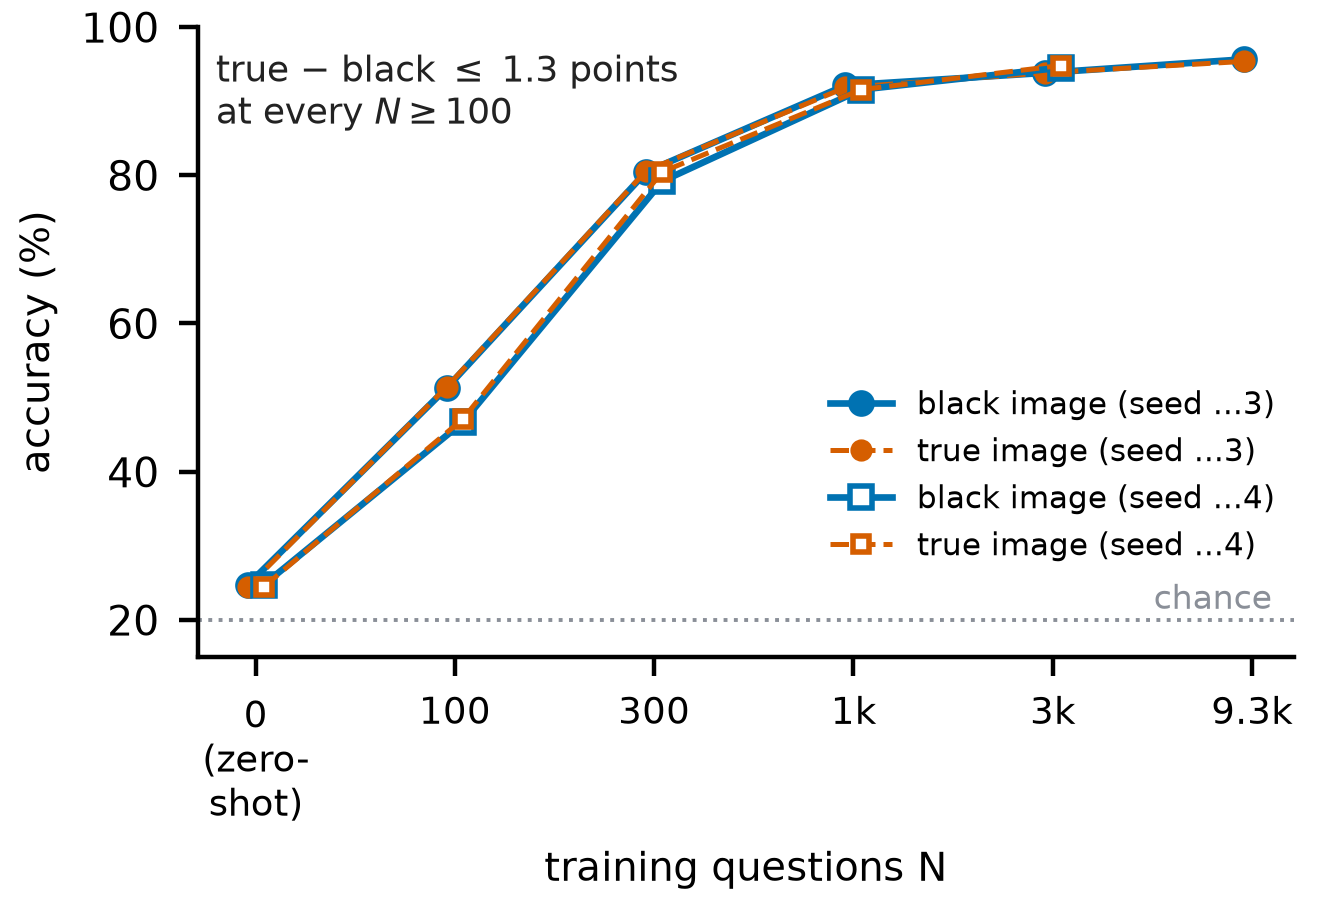
\includegraphics[width=\columnwidth]{fig/f13_curve.png}
  \caption{\textbf{Training on the benchmark installs the shortcut.} Qwen2.5-VL-3B fine-tuned on the first $N$ Med-CMR training questions (A9 recipe, two seeds), accuracy on the 711 held-out questions with a black image (solid) and with the true image (dashed); $N=0$ is zero-shot and 9.3k the full training split (one seed).}
  \label{fig:curve}
\end{figure}

\paragraph{Training on the benchmark installs the shortcut.}
Before fine-tuning, Qwen2.5-VL-3B is at chance on Med-CMR with or without the image ($24.8\%$ with a black image); after 100, 300, 1{,}000 and 9{,}277 training questions it reaches $51\%$, $80\%$, $92\%$ and $95.6\%$ with a black image, and the true-image accuracy tracks it (true minus black at most $1.3$ points at every $N\ge100$; two seeds; all three pre-registered rules held; Fig.~\ref{fig:curve}).
On OmniMedVQA the same comparison at 3B raises the black-image accuracy from $54.0\%$ to $93.2\%$, but on PMC-VQA and A-OKVQA, which have no length cue and low blind ceilings, by only $1.7$ and $0.4$ points (Supp.~Z).
Image-blind accuracy thus has two routes, the benchmark's text artifacts that training on its own split installs (the blind ceiling) and knowledge the model brings (MMMU health: $49.0\%$ without the image against a ceiling of $23.5\%$); the pre-registered 32B tests of the second were not run.

\section{Intervention: Can Headroom Be Bought Back?}
\label{sec:remedy}

If a text-side shortcut locks the decision during training, a model that is kept from using it should retain visual control.
We test this where the shortcut is planted and then on the real Med-CMR shortcut.

\paragraph{Planted shortcut: product-of-experts works.}
Product-of-experts debiasing~\cite{clark2019dont,cadene2019rubi} trains the main model on $\log p_{\rm main}+\ell_b$, where $\ell_b$ are the option log-probabilities of a text-only \emph{bias expert} trained on the \emph{other} half of the training questions; the main model alone is used at test time, and a control with weight $0$ isolates the expert.
With the cue planted at 92\% in PMC-VQA the rescued models regain an image benefit of $+16.5$, $+13.5$ and $+14.0$ points in three seeds (naive: $0.0$--$0.2$; control $+0.25$; $p<10^{-30}$), their veto boundary returns to blur 16--8 (Supp.~R) and their accuracy on cue-free questions rises from $38\%$ to $49$--$51\%$; test-time contrastive scoring does not rescue the locked model.
The cost is accuracy on cue-\emph{present} questions ($91.7\%$ to $47$--$49\%$), a gain only if the shortcut will not be available when the model is used.

\paragraph{Real shortcut: what was tried.}
On Med-CMR the same method collapses to chance accuracy because the neural expert is saturated (median probability margin $0.9995$); tempering it keeps accuracy but not the image.
Three further methods were tried with criteria fixed in advance: an explicit length-rank prior as the bias expert (LP), a penalty that makes the model uncertain when the image belongs to another case of the same modality and organ system (MU), and both (LP+MU); none met the criterion (an image effect of at least $+5$ points on the questions that the reference model found undecided, with accuracy of at least $93.5\%$; Supp.~X).
A second round used a criterion on all questions (an image effect of at least $+3$ points, accuracy of at least $88\%$), chosen after seeing the first.
A gentler penalty, UL, which lowers the probability of the correct option when the image belongs to another case, met it in all three seeds at $89.5$--$91.2\%$ accuracy; LP+MU restored image use in four of five seeds but at $77$--$80\%$ accuracy, and UL combined with the length prior collapsed.
UL's large effect against a black image ($+52$ to $+71$ points) is partly an artefact of the penalty (accuracy with a random other image is below chance, $12.7$--$16.2\%$); against a plausible wrong image of the same modality UL loses $11.5$--$11.8$ points in all three seeds, LP+MU $1.3$--$3.3$ and every other method at most $1.3$ (Supp.~Z).
So UL buys a measurable dependence on the image for $4$--$6$ points of accuracy.
The same method on Qwen2.5-VL-7B (two seeds) restores image use again (image effect $+8.0$ and $+12.0$ points, $p<10^{-25}$) at $89.6$--$90.5\%$ accuracy, about 6 points below the unpenalised model, and loses $17.5$--$17.8$ points under a plausible wrong image; its accuracy rises with sharpness, but a blur of radius 8 is no better than a black image ($77.2$ and $79.0\%$ against $82.5$ and $77.6\%$), so heavily blurred images mislead it more than no image (Supp.~Z).
A pre-registered blur test shows that at 3B this dependence is graded in sharpness but that blur 8 already recovers $81$ and $87\%$ of the gap to a black image in two of three seeds, so it rests mostly on coarse image identity (Supp.~X).

Ten attempts preceded UL (Supp.~X): three cue-removal tests, which were not evaluable, and seven interventions, which were falsified, collapsed, or exploratory. UL's criterion was chosen after these results, so its success is post hoc.
What the restored dependence is and is not. The penalised model's answers change when the image is replaced, so the dependence is measurable beyond a black image. But a plausible wrong image costs $11.5$--$11.8$ points at 3B and $17.5$--$17.8$ at 7B, which shows that much of the change tracks coarse image identity, as the blur results above also indicate, rather than the answer-relevant region. We therefore claim restored image dependence, not restored visual understanding, and the price is paid in accuracy on the same questions.

The technique is not new; what the study adds is the diagnosis that says when it is needed, a dose-controlled setting in which its effect can be attributed, and a measured price on the real shortcut.

\section{Stress Test (Robustness): Held-Out Models, Seeds and Judges}
\label{sec:general}

\paragraph{Predictions that held: held-out models and seeds.}
Before training InternVL3-2B or Qwen2.5-VL-7B on planted shortcuts we fixed the prediction from the Qwen-3B curve (benefit $13.5$, $3.4$, $0.1$ points at $d=0.25$, $0.70$, $0.92$, tolerance $\pm4$; a veto boundary at $0.25$ and none at $0.92$; a monotone decrease); both models pass all three rules in both seeds, the second of which was pre-registered before it ran (largest deviation $1.96$ points; Supp.~O).
Two further seeds of Qwen2.5-VL-3B and -7B reproduce the Med-CMR result (image effect on undecided questions $-1.0$ to $+2.5$ points, none significant) and the PMC-VQA result (gaps $+13.7$ to $+15.5$; Supp.~O); on OmniMedVQA the three families reach 98.7--98.9\% accuracy with image benefits of $+5.7$ to $+16.2$ points (Supp.~S).

\paragraph{Explanations of the boundary that failed.}
Three attempts to explain why benchmarks lock out at different strengths failed.
(i)~Because the benefit without a cue is smaller on OmniMedVQA ($+5.7$ points) than on PMC-VQA ($+13.5$), we predicted before the runs that OmniMedVQA locks out by $d=0.85$; at $0.85$ the image still adds $+3.3$ and $+2.6$ points (two seeds; the cue-uptake rule also missed by 0.05 points, a flaw of our threshold, so the amendment is not informative as written).
(ii)~A frozen one-constant hypothesis (lock-out where the log-odds evidence of the cue exceeds a constant times the mean visual log-odds gain of the cue-free model), calibrated once on Qwen-3B/PMC-VQA, fits the other PMC-VQA conditions but predicts lock-out for A-OKVQA near $d=0.9994$ (observed $0.99$; about 3 nats off) and for OmniMedVQA near $0.69$ (not locked at $0.85$).
(iii)~Without planting, the image benefit within a benchmark does not fall consistently with a question's text predictability (quintiles of an option-only classifier; Spearman $-0.2$ on PMC-VQA and A-OKVQA, $-0.7$ on OmniMedVQA, zero except in the least predictable quintile on Med-CMR; both pre-registered rules failed), because where the blind ceiling is low the classifier's confidence carries little information; the natural evidence lies between benchmarks (Fig.~\ref{fig:headroom}; correlational).
The lock-out strength is therefore a measured, benchmark-dependent property (Supp.~Z).

\paragraph{Average measures disagree.}
Across eight fine-tuned systems the accuracy drop and the visual information gain correlate at only $\rho=0.69$ (rule $\ge0.9$: failed); OmniMedVQA Qwen-3B has the information gain of PMC-VQA Qwen-3B ($0.16$ nats) but half its accuracy drop, since 64\% of its questions are text-decisive and the rest carry $+27$ points (Supp.~Z).

\paragraph{Does the challenge's faithfulness gate check the image?}
We ran the released adapter on 175 open-ended held-out cases with the true image, a black image and another case's image, and scored the traces with reproductions of the organisers' visual judge at three sizes (Qwen2.5-VL 3B, 7B, 32B; their size and prompts are unknown).
All three give black-image traces about $0.3$ of 4, because $89.7\%$ of them say the image is black or blank, and none penalises a missing image when the judge itself sees a black image or none (32B: $3.54$ and $3.39$ against $3.40$); only the 32B judge notices another case's image ($3.40\to2.36$) or trace ($1.95$).
The gate thus depends on the judge's size, and even the largest judge detects contradiction with the image, not the absence of visual evidence (Supp.~Z).

\paragraph{What did not hold.}
Failures include the image benefit on undecided questions in our fine-tuned models, a competition score, the median-margin rule, three cue-removal attempts, cue uptake and strong lock-out on A-OKVQA, the boundary shift of the position shortcut, the lock-out of InternVL3-2B at $d=0.99$, the benefit-without-a-cue predictor of lock-out and most methods on the real shortcut (Sec.~\ref{sec:remedy}).

\section{Discussion}
\label{sec:disc}

\paragraph{What the evidence supports.}
We recommend that a benchmark report its visual headroom (blind ceiling, black-image accuracy and true-image accuracy), the accuracy on counter-cue questions where a cue is known, and, for a system, its accuracy with and without the image on the text-undecided stratum with the share of text-decisive questions.

\paragraph{Limits.}
\emph{Sufficiency.} The causal claim is for a planted shortcut, not for Med-CMR's own cue; the dose-response covers two benchmarks, a held-out prediction held for two further models, but the lock-out strength differs between benchmarks and is not explained by natural variation (Sec.~\ref{sec:general}), InternVL3-2B was not locked out at $0.99$, and larger models, other shortcuts and other tasks are untested.
\emph{Real shortcut.} Ten earlier attempts did not meet their criteria (Supp.~X), UL's criterion was chosen after them, and the cue is not the only barrier; the dependence that UL induces rests mostly on coarse image identity at 3B and less so at 7B.
\emph{Method.} The faithfulness audit uses reproductions of the organisers' judge at three sizes, not their judge (size unknown); no patient identifiers exist (case-disjointness and near-duplicate filtering only; thresholds were set by an AI assistant's review of montages); the released adapter's training membership is unknown; the analyses were implemented with an AI coding assistant under the hashed pre-registration.

\paragraph{Ethics and broader impact.}
We use MedReason~2026 (CC BY-NC 4.0, as stated by its organisers), PMC-VQA (CC BY-SA 4.0), the open-access subset of OmniMedVQA, A-OKVQA, MedXpertQA-MM~\cite{zuo2025medxpertqa} and MMMU~\cite{yue2024mmmu} under their published terms, for research only; nothing here supports clinical use.
Statements about released systems describe measured behaviour on stated benchmarks and inputs, not their clinical safety or their developers' intent, and the faithfulness audit uses reproductions of a judge, not the organisers' own.

\paragraph{Conclusion.}
\emph{Demonstrated:} in our controlled setting, a nonvisual shortcut locks the decision at a benchmark-dependent strength, and a penalty restores measurable image dependence for about 4 to 6 points of accuracy, partly on coarse image identity.

\emph{Not demonstrated:} a universal lock-out law, a mechanism explaining the difference between benchmarks, or restored semantic visual understanding.

\emph{Why it matters:} VQA evaluations should report visual headroom alongside accuracy, because high accuracy alone does not show that the image contributes.

{
    \small
    \bibliographystyle{ieeenat_fullname}
    \bibliography{main}
}
\end{document}
